% Copyright (C) 2014-2016 by Thomas Auzinger <thomas@auzinger.name>

\documentclass[draft, final]{vutinfth} % Remove option 'final' to obtain debug information.

% Load packages to allow in- and output of non-ASCII characters.
\usepackage{lmodern}        % Use an extension of the original Computer Modern font to minimize the use of bitmapped letters.
\usepackage[T1]{fontenc}    % Determines font encoding of the output. Font packages have to be included before this line.
\usepackage[utf8]{inputenc} % Determines encoding of the input. All input files have to use UTF8 encoding.

% Extended LaTeX functionality is enables by including packages with \usepackage{...}.
\usepackage{amsmath}    % Extended typesetting of mathematical expression.

\usepackage{amssymb}    % Provides a multitude of mathematical symbols.
\usepackage{mathtools}  % Further extensions of mathematical typesetting.
\usepackage{blkarray}
\usepackage{microtype}  % Small-scale typographic enhancements.
\usepackage[inline]{enumitem} % User control over the layout of lists (itemize, enumerate, description).
\usepackage{multirow}   % Allows table elements to span several rows.
\usepackage{booktabs}   % Improves the typesettings of tables.
\usepackage{subcaption} % Allows the use of subfigures and enables their referencing.
\usepackage[ruled,linesnumbered,algochapter]{algorithm2e} % Enables the writing of pseudo code.
\usepackage{listings}
\usepackage{graphicx, wrapfig}

\usepackage[usenames,dvipsnames,table]{xcolor} % Allows the definition and use of colors. This package has to be included before tikz.

\newcommand{\lstfont}[1]{\color{#1}\footnotesize\ttfamily}
\lstset { %
    language=[ANSI]C++,
    backgroundcolor=\color{black!5}, % set backgroundcolor
    tabsize=4,
    basicstyle=\ttfamily\footnotesize,% basic font setting
    keywordstyle=\color{blue}\ttfamily\footnotesize,
    stringstyle=\color{red}\ttfamily\footnotesize,
    emph={
            cudaMalloc, cudaFree,
            __global__, __shared__, __device__, __host__,
            __syncthreads,
        },
    emphstyle={\lstfont{red!60!magenta}},
    breaklines=true
}
\usepackage{pgfplots}
\usepgfplotslibrary{groupplots}

\usepackage{nag}       % Issues warnings when best practices in writing LaTeX documents are violated.
\usepackage{todonotes} % Provides tooltip-like todo notes.
\usepackage{hyperref}  % Enables cross linking in the electronic document version. This package has to be included second to last.
\usepackage[acronym,toc]{glossaries} % Enables the generation of glossaries and lists fo acronyms. This package has to be included last.
\usepackage{url}

% Define convenience functions to use the author name and the thesis title in the PDF document properties.
\newcommand{\authorname}{Fabian Fuhrmann} % The author name without titles.
\newcommand{\thesistitle}{Solving Linear Equations With The GPU Architecture} % The title of the thesis. The English version should be used, if it exists.
% Set PDF document properties
\hypersetup{
    pdfpagelayout   = TwoPageRight,           % How the document is shown in PDF viewers (optional).
    linkbordercolor = {Melon},                % The color of the borders of boxes around crosslinks (optional).
    pdfauthor       = {\authorname},          % The author's name in the document properties (optional).
    pdftitle        = {\thesistitle},         % The document's title in the document properties (optional).
    pdfsubject      = {Subject},              % The document's subject in the document properties (optional).
    pdfkeywords     = {a, list, of, keywords} % The document's keywords in the document properties (optional).
}
\usepackage{tikz}

\setpnumwidth{2.5em}        % Avoid overfull hboxes in the table of contents (see memoir manual).
\setsecnumdepth{subsection} % Enumerate subsections.

\nonzeroparskip             % Create space between paragraphs (optional).
\setlength{\parindent}{0pt} % Remove paragraph identation (optional).

\makeindex      % Use an optional index.
\makeglossaries % Use an optional glossary.
%\glstocfalse   % Remove the glossaries from the table of contents.

% Set persons with 4 arguments:
%  {title before name}{name}{title after name}{gender}
%  where both titles are optional (i.e. can be given as empty brackets {}).
\setauthor{}{\authorname}{}{male}
\setadvisor{Prof. Dr. Scient.}{Jesper Larsson Träff}{}{male}

% For bachelor and master thesis:
% \setfirstassistant{Pretitle}{Forename Surname}{Posttitle}{male}
% \setsecondassistant{Pretitle}{Forename Surname}{Posttitle}{male}
% \setthirdassistant{Pretitle}{Forename Surname}{Posttitle}{male}

% Required data.
\setaddress{Franz-Graßlergasse 84 1230 Wien} 
\setregnumber{1227550}
\setdate{02}{10}{2017} % Set date with 3 arguments: {day}{month}{year}.
\settitle{\thesistitle}{Solving Linear Equations With the GPU Architecture} % Sets English and German version of the title (both can be English or German).
\setsubtitle{High Performance Computing with CUDA}{High Performance Computing with CUDA} % Sets English and German version of the subtitle (both can be English or German).

% Select the thesis type: bachelor / master / doctor / phd-school.
% Bachelor:
\setthesis{bachelor}
%
% Master:
%\setthesis{master}
%\setmasterdegree{dipl.} % dipl. / rer.nat. / rer.soc.oec. / master
%
% Doctor:
%\setthesis{doctor}
%\setdoctordegree{rer.soc.oec.}% rer.nat. / techn. / rer.soc.oec.
%
% Doctor at the PhD School
%\setthesis{phd-school} % Deactivate non-English title pages (see below)

% For bachelor and master:
\setcurriculum{Computer Engineering}{Technische Informatik} % Sets the English and German name of the curriculum.

\begin{document}

\frontmatter % Switches to roman numbering.
% The structure of the thesis has to conform to
%  http://www.informatik.tuwien.ac.at/dekanat

\addtitlepage{naustrian} % German title page (not for dissertations at the PhD School).
\addtitlepage{english} % English title page.
\addstatementpage

% \begin{danksagung*}

% \end{danksagung*}

\begin{acknowledgements*}
	In order to begin this thesis I want to thank everyone involved with my work:

	At first I want to thank Prof. Jesper Larson Träff for allowing me to write about CUDA. Even though GPU programming is not part of his lectures he did not hesitate to give me the freedom to write about this topic. Not only did he take so much time and efforts to supervise my work, but also gave me access to all the resources I needed.\\
	Without his support and collaboration this thesis would have never been as it is now.

	I also want to thank Prof. Andreas Steininger for supervising and supporting me during the lecture "Scientific Working". During this lecture I was able to rewrite a paper to get familiar with scientific writing. As he walked me through all the important steps of preparing a literature survey, writing and publishing a paper I became experienced enough to write my own thesis.

	Last but not least I want to thank my family, especially my parents, for mentally and financially supporting me during my study. They have spared no expense and efforts what so ever in order to help me with what they can.

\end{acknowledgements*}

\begin{kurzfassung}
	Datenparallele Abläufe und Algorithmen sind mittlerweile aus vielen Applikationen nicht mehr wegzudenken. Diese Bachelorarbeit befasst sich mit GPU Architektur im allgemeinen, geht aber ganz speziell auf die eigens von NVIDIA entwickelte CUDA Architektur ein. Als Beispiel für die Realisierung einer Implementierung auf einer Grafikkarte (mit CUDA Architektur) wurde das Gaußsche Eliminationsverfahren ausgewählt, welches für das Lösen linearer Gleichungssysteme benötigt wird. Mehrere parallele Lösungsstrategien wurden miteinander kombiniert um die Leistung so weit wie möglich zu verbessern. Außerdem wurde diese parallele Lösungsstrategie auch gegen eine sequentielle Implementierung auf einer CPU verglichen.
\end{kurzfassung}

\begin{abstract}
	Due to the high demand on data-parallel tasks and applications GPUs are more and more used in the high-performance-computing field. This thesis gives a short introduction to the GPU architecture. The main focus will be on the CUDA architecture, which is a highly advanced data parallel design from NVIDIA. Furthermore we try to implement the "Gaussian algorithm" with the CUDA API, using all different resources the GPU has to offer. The various parallelization techniques are not only combined in order to gain performance, but also compared to a sequential implementation on the CPU.
\end{abstract}

% Select the language of the thesis, e.g., english or naustrian.
\selectlanguage{english}

% Add a table of contents (toc).
\tableofcontents % Starred version, i.e., \tableofcontents*, removes the self-entry.

% Switch to arabic numbering and start the enumeration of chapters in the table of content.
\mainmatter



\chapter{Introduction}
	Parallel strategies for computation have been used for quite a while now. With new complex ASIC designs new challenges emerge for engineers to to not only gain performance, but also keep stability at a high level. Since modern manufacturing processes are evolving constantly and transistor size is getting smaller and smaller it has become possible to build massively parallel processors on one chip.\\
	The Graphics Processing Unit (GPU) is one these architectures. GPUs are designed to compute on very large data structures in parallel. Unlike CPUs, the GPU is not intended to handle lots of different tasks at the same time, but has other advantages over a standard processor. These advantages can significantly improve the execution time of certain applications, which gives the GPU a huge benefit compared to its predecessor.\\
	In order to execute certain programs on such a device certain Application Programming Interfaces(API) have evolved to make this step more intuitive for programmers. \textbf{The Compute Unified Device Architecture(CUDA)} \cite{Sanders:2010:CEI:1891996} is one of many APIs (such as OpenCL, OpenACC, ...) which can handle communication and workload between CPU and GPU. Thus the purpose of these frameworks is to make application developing easy and accessible for programmers.

	One can now argue that CPUs are still widely used and are far from being excluded from the market.\\
	Standard processors have always been and most likely will remain the most suitable architecture for most applications. But this thesis does not cope with the question whether GPUs are better/more future-proof than CPUs.\\
	We will give a small introduction to the GPU architecture and show the differences between the two designs.\\
	Furthermore, a well known and often used computing problem will be described and executed in parallel on a CUDA device. In this case linear equations with the Gaussian elimination method:\\
	Linear equations are widely used in various tasks and problems every day. According to \cite{Grcar2011163} similar algorithms to the Gaussian elimination method where used even in ancient China and early modern Europe and have been used ever since.\\
	It gives a brief summary over the history and modern use of linear equations. It also states the problem of efficiency scaling and why computing large input-matrices can be extremely time consuming.

	As we know the time to find the correct solution lies in $O(n^{3})$. What is more, there is a necessary "\textbf{back substitution}" (last step of the Gaussian algorithm) which has negligible execution time of $O(n^2)$. That makes the whole algorithm an order of magnitude: $O(n^3)$.\\
	Parallelizing this problem on a GPU helps to distribute the workload over the parallel cores and will hopefully significantly improve the execution time. Unfortunately, parallel computing does not reduce the order of magnitude in any kind but we will see that GPU computing can be extremely beneficial.

	Before the actual performance results are given it is necessary to explain how the measured data was collected and what the properties of the used test systems are.

	In the following chapter the measured results and alternative methods will be discussed further.\\
	In the end we will summarize the accomplishments made so far and try to come a conclusion.

	Note that this work mainly focuses on the CUDA Architecture from NVIDIA. Our implementation will use the CUDA framework too.

\chapter{Related Work}
	Even though parallel computing in general is a very wide-ranging topic, the book \cite{opac-b1133063} covers many aspects of this field. From the basic idea of parallel algorithms to programming complex cluster systems, everything is explained with examples. Even though is is mostly dedicated to CPU-application-developers, it features a section which covers the GPU architecture and gives an introduction to CUDA and OpenCL. The chapter "Algorithms for systems of Linear Equations" is extremely relevant for this thesis and gives a lot of examples on how to parallelize the Gaussian algorithm.

	Considering the CUDA architecture \cite{Sanders:2010:CEI:1891996} and \cite{Kirk:2010:PMP:1841511} explain with multiple examples how to program NVIDIA GPUs. While the first one is structured more like a tutorial and helps with understanding the basic concepts of CUDA, the second one gives an in depth look on the GPU architecture and the low level properties. Furthermore \cite{Kirk:2010:PMP:1841511} explains the history of the GPU and how these chips evolved to what they are.

	Another explanation of the architectural details is given by the report \cite{Introduction-to-GPUs}. It covers the general idea of the GPU architecture and explains some details and differences between NVIDIA and AMD chips.

	At the release of every new GPU generation, NVIDIA publishes a whitepaper with all the new features and improvements of their new chip design. One of these publication which explains the Kepler architecture in detail is \cite{nvidia_kepler_2012}.

	As this thesis not only covers hardware specific topics but also the parallel implementation of the Gaussian algorithm the following sources help to understand the mathematical background.\\
	When first digging into the topic of linear equations \cite{wiki:gaussian} gives a brief but easy to understand introduction to the Gaussian elimination method.

	More history focused but also very precise, when it comes to understanding the mathematical background, is the paper \cite{Grcar2011163} by Joseph F. Grcar. It proposes various methods and ideas for solving linear equations and even gives some of the algorithmic details.

	Another topic related paper by Gergel V. P. is \cite{parmeth}. It gives a very detailed explanation on how to parallelize linear equation systems. The author introduces different parallel implementations. Especially the so called "Row-cyclic" implementation was given a lot of attention for our own version of the parallel Gaussian elimination method.

	For porting the algorithm to the GPU architecture, not only the previously mentioned books were considered but also another interesting concept of pipelining the back substitution, which is the last step of the Gaussian algorithm. In \cite{pipelinecomp} the author introduces this idea to the CPU and is able to save time, though \cite{opac-b1133063} claims that back substitution in general is considered to be very difficult to improve.

\chapter{State Of The Art: The GPU Architecture}
	According to \cite{Kirk:2010:PMP:1841511}, GPUs evolved from graphics pipelines in the early 80s. Due to the constantly higher demand for faster graphics calculations, GPU technology had to change from a simple pipeline system to complex array of parallel processing cores. %s.23
	This type of arrangement can be first seen in 2006.\\
	In this section we will discuss the modern GPU internal and compare it to a typical CPU. Furthermore an introduction to NVIDIA's CUDA architecture and its API will be given.

	\section{The GPU Architecture}
		\begin{figure}[!ht]
			\centering
			\begin{subfigure}[t]{.5\textwidth}
				\centering
				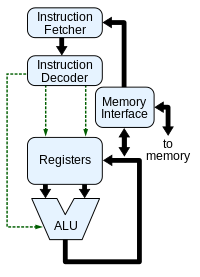
\includegraphics[width=0.4\linewidth]{images/200px-CPU_block_diagram.png}
				\caption{A block diagram of a simple CPU architecture Source: \cite{wiki:CPU_block_dia}}
				\label{fig:cpu arch}
			\end{subfigure}

			\begin{subfigure}[t]{.9\textwidth}
				\centering
				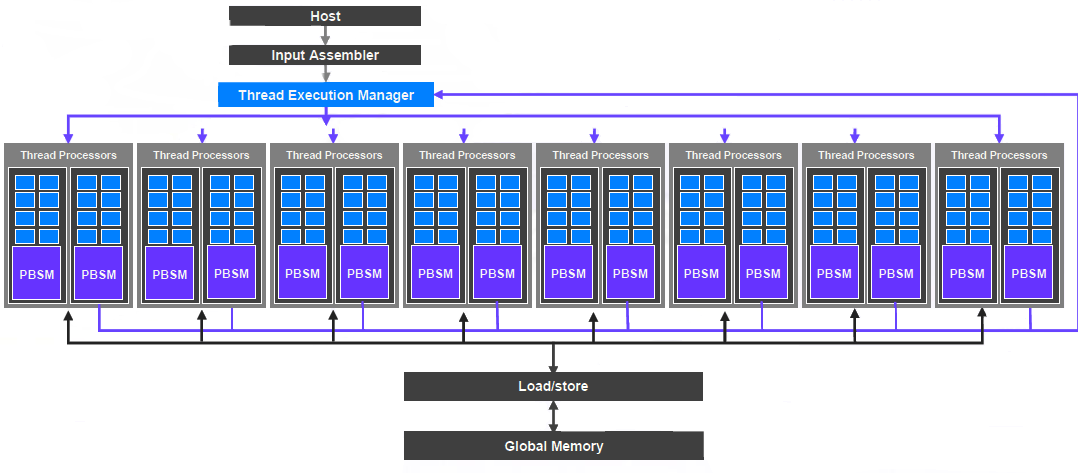
\includegraphics[width=\linewidth]{images/GPU-architecture-2.png}
				\caption{A block diagram of a simple GPU architecture which consists of 8 SMs(Thread Processors). Inside of each SM the parallel ALUs are located. Source: \cite{tatourian}}
				\label{fig:gpu arch}
			\end{subfigure}

			\caption{Comparison between CPU and GPU}
			\label{fig:gpu_vs._cpu}
		\end{figure}

		The modern GPU architecture differs very much from the typical CPU design. While standard processors are built to schedule multiple tasks at the same time, the GPU is meant to handle lots of data in parallel. This design allows the architecture to process massive amounts of data at the same time. We can imagine that thousands of Arithmetic Logic Units(ALU) are performing the same arithmetic operations on given data in parallel. So one can see the potential performance improvement over the CPU in certain tasks.

		\subsection{Streaming Multiprocessors}
			\begin{wrapfigure}{l}{0.25\textwidth}
				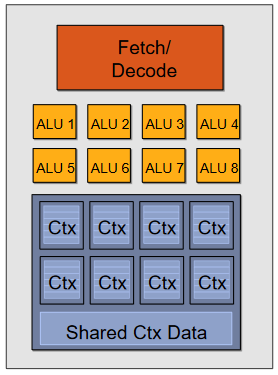
\includegraphics[width=0.2\textwidth]{images/SM.PNG}
				\caption{A simple s draft of a SM Source: \cite{Introduction-to-GPUs}}
				\label{fig:SM}
				\vspace{-110pt}
			\end{wrapfigure} 
			Figure ~\ref{fig:gpu_vs._cpu} shows the architecture of a modern GPU compared to the CPU. On a typical CPU chip each core gets an independent instruction stream, however this is not efficient and easy to handle for a data-parallel application. So designers came up with a different idea: On a GPU only one instruction stream is used across many ALUs.

			It can be noted that the different cores on the Graphics-chip are grouped together, while on the CPU each core is totally independent of the others. These groups are called \textbf{Streaming Multiprocessors(SM)}. All threads in a SM share the same instruction stream and a piece of very fast memory(cache) which can be used to exchange data inside the multiprocessor.

		\subsection{Global Memory}
			Every SM is connected through the \textbf{global memory}. This is a very large memory (today multiple gigabytes) where the input data can be fetched from the SM. In the CPU architecture this type of memory would be called Random Access Memory (\textbf{RAM}), because they have very much the same purpose.\\
			In \cite{Kirk:2010:PMP:1841511} the author explains that this type of memory is built with Dynamic Random Access Memory (\textbf{DRAM}) which is much slower compared to other implementations. Fortunately it is common for GPUs to have dedicated shared memory inside of a SM. This can and should be used for quickly exchanging data between cores.

			\subsubsection{Constant Memory}
			Constant Memory is, as the name may indicate, a read only section which is available for every SM. The books \cite{Sanders:2010:CEI:1891996} and \cite{Kirk:2010:PMP:1841511} explain that by using read only memory we can save bandwidth compared to the standard Global Memory.

		But the previously mentioned differences are not the only variations featured by those two architectures. They also differ in:

		\begin{itemize}
			\item \textbf{Clock Speed:} CPUs normally have a much higher frequency. (multiple gigahertz, while to this day a high end GPU runs with ~1.5GHz)

			\item \textbf{Branch Prediction:} GPUs in general do not support branch prediction, however CPUs do have advanced features which allow them to predict possible outcomes of a branch.

			\item \textbf{Cache:} CPUs have multiple levels of cache which is typically much larger than on the GPU.
		\end{itemize}

		\subsection{BUS-System}
			In order to exchange data between the \textbf{Host(CPU with RAM)} and the \textbf{Device(Graphics card)} GPUs use a wide bus system, which is briefly explained in \cite{Introduction-to-GPUs}.\\
			Data which will be used for computing on the graphics card has to be moved back and forth from the RAM to the global memory in order to execute instructions on it. One has to think of programming two separate systems which are connected through the bus.\\
			Therefore none of these systems can fetch the other one's data if it hasn't been exchanged.\\
			In \cite{Introduction-to-GPUs} it is made clear that even though we can send over a hundred GB/s through the PCI-Express bus, latency still comes into play if the rate of requested data is too high. So every developer has to consider these limitations and should instead use the on-chip communication and storage features as far as possible.

	\section{The CUDA Architecture}
		This section will mainly focus on NVIDIAs GPU architecture based on the previously discussed concept of using multiple parallel Streaming Multiprocessors. NVIDIA has made several improvements to their GPUs in order to gain power efficiency and performance. Even for parallel application development they simplify parallel programming with their widely used CUDA API.\\
		Due to limitations of this thesis it is not possible to cover the CUDA architecture in such detail. Every time NVIDIA releases a new product generation they further improve the architecture. The description below covers all the basic ideas and design principles which have not changed within the last three iterations.

		\subsection{Hardware}
			\begin{figure}[!ht]
			    \centering
			    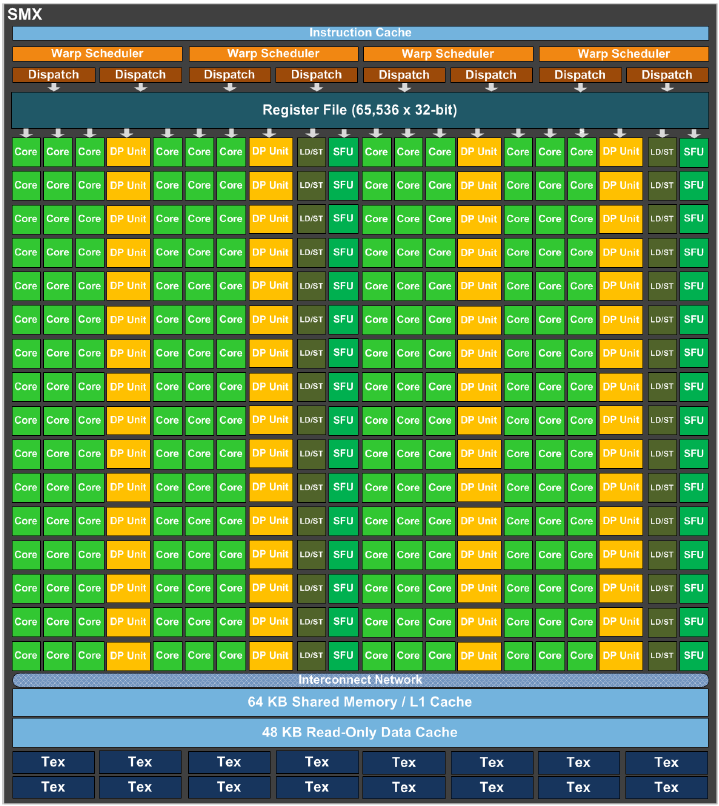
\includegraphics[width=0.8\textwidth,keepaspectratio=true]{images/CUDA-SMX-Unit.png}
			    \caption{Block diagram of a SMX (Streaming Multiprocessor). Cudacores are divided into Warps which get executed by the Warp Scheduler. The cores inside of the SMX can access the Shared Memory, Read-Only Cache and the Texture Memory. Source: \cite{nvidia_kepler_2012}}
			    \label{fig:smx}
			\end{figure}
			The diagram ~\ref{fig:smx} includes every of the following hardware components which will be covered in this section.

			\subsubsection{SMX, SMM, ...: A "Next Gen" SM}
				Since NVIDIA's \textbf{Kepler} architecture new terms for the Streaming Multiprocessor were introduced every generation. They refer to the Kepler-SM as "\textbf{SMX}". NVIDIAs white-paper \cite{nvidia_kepler_2012} about the Kepler architecture explains how this type of architecture evolved from their previous design \textbf{Fermi}. Even though Kepler is not the latest generation anymore and even falls (to this date, \cite{nvidia_kepler_2012}) 2 iterations behind, it is still widely used in the field. Furthermore there have not been any major changes to the design principles since this architecture.

				But what makes the SMX unique compared to a standard SM? We will later see that NVIDIA additionally divides the array of cores inside the SM into smaller segments, called "\textbf{warps}".

			\subsubsection{CUDA Cores}
				The term CUDA Core very frequently occurs when dealing with NVIDIAs GPU architecture. It is one of the parallel ALUs located on each SM. These cores are aligned in warps, which are visible in ~\ref{fig:smx} and explained in the following paragraph.

			\subsubsection{Warps}
				As one can see in ~\ref{fig:smx} Cuda cores are divided into smaller segments which an be somewhat independent from one another. As already mentioned NVIDIA calls these segments "\textbf{warps}"\\
				Both \cite{Introduction-to-GPUs} and \cite{nvidia_kepler_2012} show that each warp has its own dedicated \textbf{Fetch/Decode} stage but share the same instruction-cache, shared memory, ... In simple words, every instruction in a warp is shared between all cores inside.\\
				This is basically the concept of data-parallelism, which does not mean that every CUDA-core is computing on the same data. Every core uses its register file where it can fetch its own data on which the instruction is executed.\\
				This could lead to a potential slow down when using branch instructions such as "\textbf{if}", "\textbf{while}" and "\textbf{for}": According to \cite{Kirk:2010:PMP:1841511}, when some of the threads in \textbf{one} warp execute one path of a branch while the others want to take the another route, it is necessary that these steps have to be sequential because we can only \textbf{fetch one instruction for each warp at a time}. Unfortunately it is now the compiler's job to do certain optimizations in order to fight against these issues.\\
				An overview on our attempt to distribute data over one SM is given in ~\ref{subsec:vector_par}.

			\subsubsection{Warp Scheduler}
				A modern NVIDIA SM features several Warp Schedulers for selecting and activating the decided warps. According to \cite{nvidia_kepler_2012} each scheduler can set one warp as active and fetches one independent instruction per \textbf{dispatch unit} in a cycle.

			\subsection{Memory inside of the SM}
				As we briefly discussed in the previous section, having memory inside of a SM is indispensable for buffering, synchronizing and communication. The CUDA architecture features the following types of memory for a SM:

				\begin{itemize}
					\item \textbf{Shared Memory:} This is a very fast memory which can be allocated by the developer. Every change/allocation can be seen by every thread in a SM.

					\item \textbf{Texture Units:} Texture Memory is another feature CUDA has to offer. It is a read-only cache and should be used when threads have to access certain data with a high period. According to \cite{nvidia_kepler_2012} and \cite{Sanders:2010:CEI:1891996} the hardware can access texture regions extremely fast so it has a lot of benefits compared to global memory.

					\item \textbf{Read-Only Data Cache:} This was part of the Kepler generation but is not featured in newer versions of the architecture.

					\item \textbf{Instruction Cache/Buffer:} Every incoming instruction will be stored here until it is fetched by the warp scheduler.
				\end{itemize}

		\subsection{Software}
			When working on a CUDA application, NVIDA differs between two kinds of code: \textbf{Host-} and \textbf{Device} code. The first one gets executed by the CPU and the other one by the Graphics card. As we have said before, we have to think of separate systems which are connected through the bus when programming GPUs. This whole concept of how to program GPU-devices is also explained with more detail in \cite{Sanders:2010:CEI:1891996} and \cite{Kirk:2010:PMP:1841511}. Both books were taken as an inspiration for this section.\\
			When the Program Counter of the CPU stops at a device section(device code) of the code, a so called "\textbf{Kernel function}" gets launched and every following instruction is now executed on the CUDA device. It is possible to launch multiple Kernels in a row but only one is executed at a time. The scheduling works according to the \textbf{FIFO} principle as shown in figure ~\ref{fig:kernel_launch}.\\
			When developing a CUDA application the developer has to specify how many Streaming Multiprocessors and Threads should start.

			\begin{figure}[!ht]
			    \centering
			    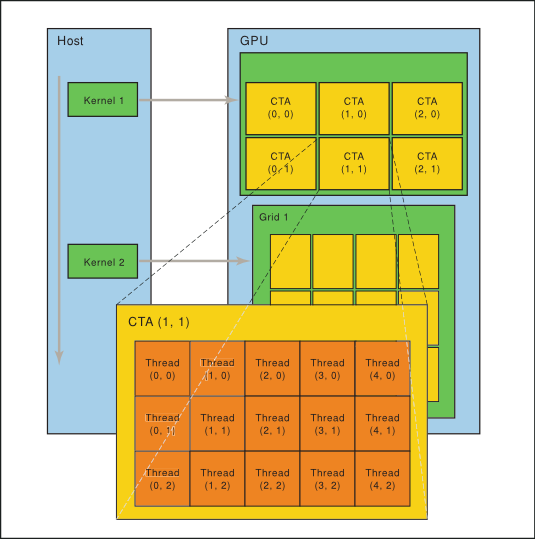
\includegraphics[width=0.5\textwidth,keepaspectratio=true]{images/thread-batching.png}
			    \caption{Brief illustration of a Kernel function which launches threads inside blocks Source: \cite{toolkit}}
			    \label{fig:kernel_launch}
			\end{figure}

			\subsubsection{Blocks}
				NVIDIA calls each SM a \textbf{Block}. These blocks are arranged into a multidimensional array by software and will be executed in parallel. However, if more blocks than available SMs get launched at the same time, some of them will have to wait until others have finished their work. Launching blocks is very efficient, a developer should not worry about the number of parallel blocks.\\
				Unfortunately, parallel SMs are not meant to be synchronized because of the potential deadlock, which can occur with launching a higher number of blocks than SMs. However, there is a way a developer can schedule/synchronize blocks, but this is only possible through the use of \textbf{atomic} operands. The use of atomics is very inefficient and they should only be used with caution. We will later see that these operants will produce so much unnecessary overhead that a proposed implementation, which we would consider as theoretically efficient, will not gain any performance compared to a much simpler/naiver one.

			\subsubsection{Threads}
				Threads can be seen as, the actual cores which do the actual work. One can think of these threads as packed together in a block where developers can decide how many threads are launched per SM. Like with blocks, we can arrange each thread in an array of multiple dimensions. This leaves a lot of freedom to the developer and helps to keep the implementation short and well structured.\\
				Again it is \textbf{not} important to pay attention if the number of threads exceeds the amount of CUDA cores. As mentioned before every CUDA core is capable of executing multiple threads. However due to software limitations there is a maximum number on how many threads can be set for each block. According to \cite{Sanders:2010:CEI:1891996} passing this limit could cause potential errors and bugs.

				Now that we know what threads are, it is necessary to discuss what other features threads have to offer:\\
				Unlike blocks, threads do offer the feature of \textbf{barrier synchronization}. When using this function each thread will wait until all have passed the barrier.\\
				Another feature is the usage of shared memory which was previously mentioned in the \textbf{hardware section}. A developer should consider using this memory if possible, because taking the longer path over the Global Memory is much slower and inefficient.

\chapter{Solving Linear Equations with CUDA}
	In this section we focus on porting a well known algorithm to the CUDA architecture. As mentioned in the introduction, we want to evaluate linear equations with the \textbf{Gaussian elimination} method. Unfortunately, the standard procedure is originally sequential, but we will see that we can adapt this algorithm in order to parallelize this problem.

	\section{Gaussian Elimination In General}
		We can think of this problem as $A \times \vec{x} = \vec{b}$ where we have to find the Vector $\vec{x}$, which is the missing part for our equation.\\
		It is widely known that this procedure takes multiple linear equations in form of either 2 $N\times N$ plus $N\times 1$ or one $N\times (N+1)$ matrices if you see the $\vec{b}$ vector as part of the matrix. 
		In the first step matrix $A$ has to be converted in an upper triangle form with \textbf{forward elimination} followed by a \textbf{back-substitution}. This last step creates solution vector $\vec{x}$ which we wanted to find in the first place.\\
		As \cite{Grcar2011163} and \cite{wiki:gaussian} report, the Gauss matrix $M$ allows several operations:
		\begin{itemize}
			\item Swapping rows
			\item Swapping columns
			\item Multiplying a row with $\alpha \epsilon \mathbb{R} | \alpha \neq 0$
			\item Subtracting/Adding one row from/to another.
		\end{itemize}
		The following formulas should give brief overview on how this process works. However if further reading into this topic is necessary, the article \cite{wiki:gaussian} sums it up just fine.

		Equation before Gaussian elimination:
		\begin{equation}
			\begin{pmatrix}
			 a_{0} &  a_{1} & a_{2} \\ 
			 a_{3} &  a_{4} & a_{5} \\ 
			 a_{6} &  a_{7} & a_{8} 
			\end{pmatrix}
			\begin{pmatrix}
			 x_{0}\\ 
			 x_{1}\\ 
			 x_{2}
			\end{pmatrix}
			=
			\begin{pmatrix}
			 b_{0}\\ 
			 b_{1}\\ 
			 b_{2}
			\end{pmatrix}
		\end{equation}

		Equation after forward elimination:
		\begin{equation}
			\begin{pmatrix}
			 \acute{a_{0}} &  \acute{a_{1}} & \acute{a_{2}} \\ 
			 0           &  \acute{a_{4}} & \acute{a_{5}} \\ 
			 0           &  0           & \acute{a_{8}} 
			\end{pmatrix}
			\begin{pmatrix}
			 x_{0}\\ 
			 x_{1}\\ 
			 x_{2}
			\end{pmatrix}
			=
			\begin{pmatrix}
			 \acute{b_{0}}\\ 
			 \acute{b_{1}}\\ 
			 \acute{b_{2}}
			\end{pmatrix}
		\end{equation}

	\section{Attempt To Parallelize The Problem}
	\label{sec:parallelize_prob}
		Most algorithms have to be adapted in order to be executed in parallel. As we will see in our solution strategies on the GPU there are often multiple approaches on how to distribute a problem to many processing cores.

		In the introduction of this thesis we mentioned that the Gaussian elimination method has an order of magnitude $O(n^3)$, which indicates that this algorithm needs 3 nested loops in order to execute.\\
		This can stretch the execution time pretty fast and with a few thousand elements in a row a sequential core can take multiple hours.\\
		Therefore we want to discuss this problem further.

		\begin{algorithm}[!ht]
			\SetKw{BreakFor}{break for}
			\KwIn{A matrix $M_{i,j}$ which includes matrix $\mathbf{A} = (a_{ij})$ and vector $\vec{b}$}
			\KwOut{An upper triangular matrix $M'_{i,j}$}
			\BlankLine

			\For{$i\leftarrow 1$ \KwTo $i$}{
				$div\leftarrow M[k][k]$

				\For{$x\leftarrow 1$ \KwTo $j$}{
					$M[i][x]\leftarrow M[i][x]/div$ %M[x] = M[x]/div\;
				}

				\For{$y\leftarrow k$ \KwTo $j$}{
					$factor\leftarrow M[y+1][k]$ %\factor = M[y+1][k]\;

					\If{$f = 0$}{
						continue
					}

					\For{$x\leftarrow 1$ \KwTo $j$}{
						$M[y+1][x] \leftarrow M[y+1][x] - M[k][x] * f$
					}
				}
			}

			\caption{Gauss algorithm: Forward elimination}
			\label{alg:forward_elem}
		\end{algorithm}

		As we can see in Alg:~\ref{alg:forward_elem} there is another path in the algorithm which adds to the execution time. The second $for$ loop has an order of magnitude $O(n^2)$. Even though the practical execution time is $O(n^3)$ we still try to parallelize every loop as far as possible.

		But let's take a look at the \textbf{back substitution}.
		\begin{algorithm}[!ht]
			\SetKw{BreakFor}{break for}
			\KwIn{Upper triangular matrix $M_{i,j}$ which includes matrix $\mathbf{A} = (a_{ij})$ and vector $\vec{b}$}
			\KwOut{Vector $\vec{x}$ which contains the solutions}
			\BlankLine

			\For{$y\leftarrow j$ \KwTo $1$}{
				$t \leftarrow M[y][i]$ %\t = M[y][i]\;
				$k \leftarrow i$ %\x = i-1\;

				\While{$M[y][k] \neq 1$}{
					$t \leftarrow t - M[y][k]*x[k]$ %t = t-M[y][k]*x[x]\;

					$k \leftarrow k-1$
				}

				$x[k] \leftarrow t$ %x[x] = t\;
			}

			\caption{Gauss algorithm: Back substitution}
			\label{alg:back_subst}
		\end{algorithm}

		In Alg:~\ref{alg:back_subst} it is noticeable that the back substitution unfortunately does not have a linear runtime. This computation lies in $O(n^2)$, so we can say that our final order of magnitude is $O(n^3)$. In the long-run the cubic execution time will make the quadratic paths irrelevant but in this thesis we pay attention to all execution paths because there is a lot of potential room for parallelization.

		But which attempts can be made in order to use a parallel architecture for our problem? In order to try various implementation strategies a few different sources were considered for other parallel implementations:

		\subsection{Vector parallelization}
		\label{subsec:vector_par}
			The book \cite{Sanders:2010:CEI:1891996} introduces a data parallel strategy where a computation on a large vector has to be made. They divide the vector into parts so that each thread gets its own dedicated section of the vector so that all workers execute the same instruction on different data.\\
			This method can be used for performing several tasks on the horizontal lines of the Gaussian matrix.

		\subsection{Parallel Row-Cyclic implementation}
			The book \cite{opac-b1133063} has a dedicated chapter about various procedures for finding the correct solution vector $\vec{x}$ in linear systems.\\
			When talking about a row-cyclic implementation we can think of horizontal "stripes" which represent parts of the input matrix. Each of these stripes is owned by a processor which computes on his section until it has to exchange information with is neighbor core. This idea is also demonstrated in paper \cite{parmeth}.

		\subsection{Sum-reduction in back substitution}
			The idea of sum reduction is to improve sequential summation by using half as many cores as values. Each core adds 2 values together. After each summation the number of cores are cut in half and proceed further with the left values.\\
			The book \cite{Sanders:2010:CEI:1891996} presents a clever solution (\textbf{sum-reduction}) which we can use for our implementation:

			\begin{figure}[!ht]
			    \centering
			    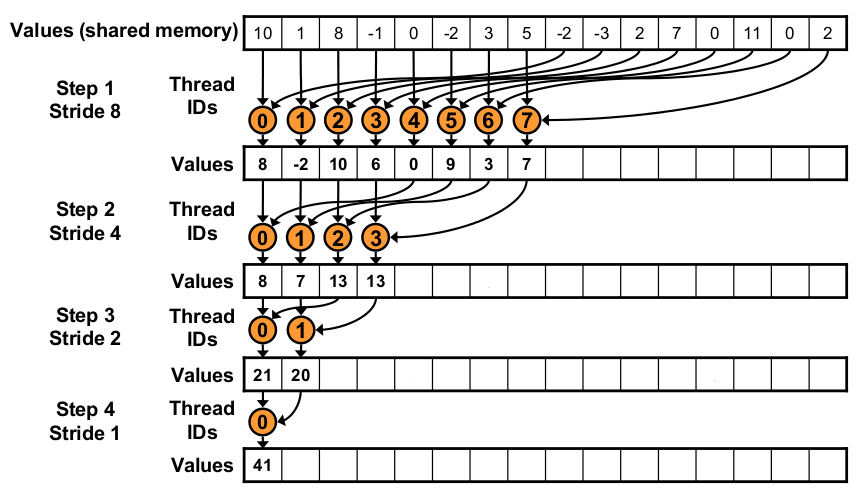
\includegraphics[width=0.5\textwidth,keepaspectratio=true]{images/tUUzE.png}
			    \caption{Illustration of Summation Reduction Source: \cite{stack:overflow_2014}}
			    \label{fig:summ_red}
			\end{figure}

		\subsection{Using a pipeline for back substitution}
			The Paper \cite{pipelinecomp} introduces the idea of pipelined back substitution. The main idea is to divide the upper triangular gauss matrix into stages where each stage passes its computed values to the next stage which waits for this data. One can benefit from this idea as horizontal lines can be partially computed in advance even though back substitution is considered to be inherently sequential. \cite{opac-b1133063}

	\section{Parallelization with CUDA}
		With the previously discussed ideas for parallelization we can now start putting the puzzle together.\\
		Because of what we know now about threads and blocks, it is important to think about where to use what. For example it is known that barrier synchronization is not allowed outside Threadblocks, so we should consider just using them where they could never interfere with each other.

		The proposed CUDA implementation will use every idea which was covered in the previous section. We start by parallelizing every iteration on the horizontal lines of the input matrix $M_{i,j}$.\\

		\subsection{Parallelizing with threads}
			In GPU computing thread-parallelization can be done very cheaply by assigning every thread in a block to an index of the matrix. As mentioned before, there are a lot of theoretical parallel threads inside a SM, so even very large loops can be cut down very efficiently:

			The code below represents the improved version of the pivoting of the current row in the matrix. $tid$ represents the thread id. One can see that we have to increment $tid$ every time the array is still too long. This approach is also used in \cite{Sanders:2010:CEI:1891996}.
			\begin{lstlisting}
__device__ void divide(double *M_row, int length, int index){
	int tid = threadIdx.x + index;

	double div = M_row[index];
	__syncthreads();
	while (tid < length){
		M_row[tid] /= div;
		tid += blockDim.x;
	}
}
			\end{lstlisting}

			Here we have adapted basically the same idea. The pivot row \textbf{M\_row} is being subtracted from the current row \textbf{M\_row\_current}.
			\begin{lstlisting}
__device__ void subtract(double *M_row, double *M_row_current, int length){
    int tid = threadIdx.x;
	while (tid < var_count+1)
	{
		M_row_current[tid] -= M_row[tid] * factor;
		tid += blockDim.x;
	}
}
			\end{lstlisting}

			But there is still another implementation left where horizontal iterations are used. The back substitution sums all the factorized row elements and subtracts them from the corresponding element in the $\vec{b}$ vector. But therefore it is not that easy because all the threads working on the sum have to work together on the sum instead of just working independently on their own space.\\
			
			The idea behind this is to use a shared memory section which holds the values for the summation. The memory has to be large enough for every worker to have one slot to put its data. Now it is necessary to iteratively halve the number of threads which are allowed to compute on the shared section. Every thread has now 2 values to sum. This whole process is repeated until just one worker is left. His job is to compute the sum by adding the last two values together.\\
			Even though half of the parallel threads are lost after every iteration it is still more efficient than the sequential method. With one core a summation has a complexity of $O(n)$ steps while the summation reduction finishes in $O(\log(t))$ steps (t = number of threads):

			\begin{lstlisting}
#define ROUND_UP(N, S) (N%S == 0) ? N/S : N/S+1
__global__ void calc_solutions(double *d_matrix, size_t pitch,
	int var_count, double *d_solution){
	int tid = blockDim.x*blockIdx.x + threadIdx.x,
		count = 0;
	for (int y = var_count-1; y >= 0; --y)
	{
		int tid_temp = tid + (var_count - blockDim.x);
		double *temp_p = (double*)((char*)d_matrix + y * pitch);
		double temp = 0;
		extern __shared__ double cache[]; //shared memory
		__syncthreads();

		//push data to shared memory. compress if necessary.
		while(BETWEEN(tid_temp, (var_count-1) - count, var_count)){
			temp += temp_p[tid_temp]*d_solution[tid_temp];
			tid_temp -= blockDim.x;
		}

		cache[threadIdx.x] = temp;
		__syncthreads();

		int i = ROUND_UP(blockDim.x, 2);

		//cite cuda by example page 85
		while(i > 1){
			if (threadIdx.x < i)
			{
				if (threadIdx.x +i < blockDim.x)
				{
					cache[threadIdx.x] += cache[threadIdx.x +i];
					cache[threadIdx.x +i] = 0;
				}
			}
			__syncthreads();

			i = ROUND_UP(i, 2);
		}

		if(threadIdx.x == 0){
			if (i == 1)
				cache[0] += cache[1];
			d_solution[var_count-count-1] = temp_p[var_count] - cache[0];
		}

		__syncthreads();

		count++;
	}
}
			\end{lstlisting}
			It can be seen that the algorithm has to check if there are more values to sum than available threads. In order to compute on the shared memory we have to first compress the horizontal elements, so that they can be positioned in their slot. This can be easily done by computing a partial sum over the horizontal elements with each thread and then placing them into the shared memory.

			\subsubsection{Complexity (Using Threads)}
				As previously described in ~\ref{sec:parallelize_prob} the Gaussian algorithm has a complexity of $O(n^3)$. As we have seen before we can parallelize every loop where we use a row-wise iteration over the elements in the matrix. Because we simply distribute the elements of every row $M_i$ evenly over the threads $t$, we can define our new complexity as: $O(\frac{n^3}{t})$.

		\subsection{Parallelization with Streaming Multiprocessors}
			Now as we proceed further with our implementation, we are still missing a proper usage of the Streaming Multiprocessors for gaining performance.

			One simple, naive approach would be to just use more threads inside the other blocks to parallelize the horizontal rows, but as discussed before NVIDIA does not provide any native way of block synchronization. We have also discussed that using atomics will result in an extremely heavy overhead. Therefore another form of workload distribution has to be considered:
			\begin{figure}[!ht]
			    \centering
			    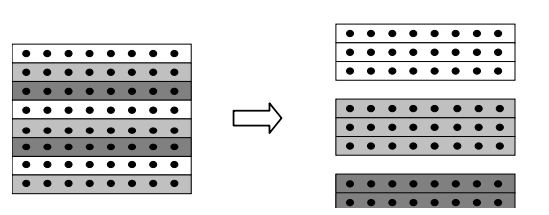
\includegraphics[width=0.7\textwidth,keepaspectratio=true]{images/block_dist.PNG}
			    \caption{Cyclic striped scheme distributed onto processors. Source: \cite{parmeth}}
			    \label{fig:row_dist}
			\end{figure}

			As blocks are not allowed to interfere with each other, one possible solution is to use some form of "Parallel Row-Cyclic" implementation:\\
			The strategy we are using works a lot like a \textbf{divide and conquer} algorithm. The matrix will be spread in stripes across the SMs. As soon as a block knows which part of the matrix it owns, it starts with the forward elimination until it reaches the end of its own section.\\
			Furthermore the matrix is sill \textbf{not} in the desired upper-triangular form even if all Streaming Multiprocessors have finished their job.\\
			The idea is to launch a new Kernel with \textbf{fewer} blocks than before and start with the whole process again. This goes on until there is just one single block left. As long as there are fewer blocks than in the previous iteration, the matrix will always end up in the upper-triangular form.\\
			The main idea behind this concept is that with every new kernel launch there are fewer horizontal-line-subtractions necessary because of the preliminary work. But we will explain this technique further as we move on with this section.\\

			As CUDA does not provide any fancy functions like MPI does, we just avoid passing messages between SMs. As already discussed every block computes on his own part of the matrix and will not be interfered. How the work distribution works in detail can be obtained from Figure: ~\ref{fig:row_dist}.

			\begin{lstlisting}
__global__ void naive_aproach_divide_n_merch_cuda(double *M, size_t pitch,
	int length){
	int tid = threadIdx.x;
	int block_inc = gridDim.x;

	int count = 0;
	for (int i = blockIdx.x; i < length; i += block_inc)
	{
		double *row = (double*)((char*)M + i * pitch);
		divide_multi(row, length+1, count);
		for (int y = i; y < length-block_inc; y += block_inc)
		{
			double *row_y = (double*)((char*)M + (y+block_inc) * pitch);
			double factor = row_y[count];
		    __syncthreads();
			if (factor == 0) //ignore every row below this one
				break;

		    subtract(row, row_y, length);
		}
		
		count++;
	}
}
			\end{lstlisting}

			But now it has to be explained, why this method can reduce the execution time. Compared to the previous optimization technique, where parallelization was implemented just with threads, this procedure may be a bit more difficult to understand:

			\subsubsection{A Small Example}
			\label{ssec:example}
				The following example illustrates the idea behind our implementation. Every $X$ represents a non zero element of the matrix $M_{i,j}$. For this example we used a $6 \times 6$ Matrix where each row is assigned to one of 3 SMs (according to Figure: ~\ref{fig:row_dist}). Each SM performs a forward elimination on its own segment:
				\begin{equation}
					\begin{aligned}
						\begin{blockarray}{cccccccc}
							\begin{block}{c(ccccccc)}
							\scriptscriptstyle{a} & X & X & X & X & X & X &| X \\ 
							\scriptscriptstyle{b} & X & X & X & X & X & X &| X \\ 
							\scriptscriptstyle{c} & X & X & X & X & X & X &| X \\ 
							\scriptscriptstyle{d} & X & X & X & X & X & X &| X \\ 
							\scriptscriptstyle{e} & X & X & X & X & X & X &| X \\ 
							\scriptscriptstyle{f} & X & X & X & X & X & X &| X \\
							\end{block}
						\end{blockarray}
						\xrightarrow[]{\text{pass to 3 SMs}}
						\begin{blockarray}{cccccccc}
							\begin{block}{c(ccccccc)}
								\scriptscriptstyle{a} & X & X & X & X & X & X &| X \\ 
								\scriptscriptstyle{d} & X & X & X & X & X & X &| X \\
							\end{block}
						\end{blockarray}
					\end{aligned}
				\end{equation}
				Each SM now computes on its own dedicated piece (left).			After each block terminates we can see the current status of the Matrix on the right:
				\begin{equation}
					\begin{aligned}
						\begin{blockarray}{cccccccc}
							\begin{block}{c(ccccccc)}
								\scriptscriptstyle{a} & 1 & X & X & X & X & X &| X \\ 
								\scriptscriptstyle{d} & 0 & 1 & X & X & X & X &| X \\ 
							\end{block}
						\end{blockarray}
						\xrightarrow[]{\text{$1^{st}$ iteration (3 cores)}}
						\begin{blockarray}{cccccccc}
							\begin{block}{c(ccccccc)}
								\scriptscriptstyle{a} & 1 & X & X & X & X & X &| X \\ 
								\scriptscriptstyle{b} & 1 & X & X & X & X & X &| X \\ 
								\scriptscriptstyle{c} & 1 & X & X & X & X & X &| X \\ 
								\scriptscriptstyle{d} & 0 & 1 & X & X & X & X &| X \\ 
								\scriptscriptstyle{e} & 0 & 1 & X & X & X & X &| X \\ 
								\scriptscriptstyle{f} & 0 & 1 & X & X & X & X &| X \\
							\end{block}
						\end{blockarray}
					\end{aligned}
				\end{equation}
				This step now gets repeated with fewer cores, that means that each SM gets a larger section of the Matrix.
				If we would not decrease the amount of active SMs the Matrix would not change its appearance:
				\begin{equation}
					\begin{aligned}
						\begin{blockarray}{cccccccc}
							\begin{block}{c(ccccccc)}
								\scriptscriptstyle{a} & 1 & X & X & X & X & X &| X \\ 
								\scriptscriptstyle{b} & 1 & X & X & X & X & X &| X \\ 
								\scriptscriptstyle{c} & 1 & X & X & X & X & X &| X \\ 
								\scriptscriptstyle{d} & 0 & 1 & X & X & X & X &| X \\ 
								\scriptscriptstyle{e} & 0 & 1 & X & X & X & X &| X \\ 
								\scriptscriptstyle{f} & 0 & 1 & X & X & X & X &| X \\
							\end{block}
						\end{blockarray}
						\xrightarrow[]{\text{pass to 2 SMs}}
						\begin{blockarray}{cccccccc}
							\begin{block}{c(ccccccc)}
								\scriptscriptstyle{a} & 1 & X & X & X & X & X &| X \\ 
								\scriptscriptstyle{c} & 1 & X & X & X & X & X &| X \\ 
								\scriptscriptstyle{e} & 0 & 1 & X & X & X & X &| X \\ 
							\end{block}
						\end{blockarray}
					\end{aligned}
				\end{equation}
				As we can see in the matrix above we can skip the subtraction for the third line because it already contains a zero at the beginning. After each SM has finished its own forward elimination the Matrix looks like this:
				\begin{equation}
					\begin{aligned}
						\begin{blockarray}{cccccccc}
							\begin{block}{c(ccccccc)}
								\scriptscriptstyle{a} & 1 & X & X & X & X & X &| X \\ 
								\scriptscriptstyle{c} & 0 & 1 & X & X & X & X &| X \\ 
								\scriptscriptstyle{e} & 0 & 0 & 1 & X & X & X &| X \\ 
							\end{block}
						\end{blockarray}
						\xrightarrow[]{\text{$2^{nd}$ iteration (2 cores)}}
						\begin{blockarray}{cccccccc}
							\begin{block}{c(ccccccc)}
								\scriptscriptstyle{a} & 1 & X & X & X & X & X &| X \\ 
								\scriptscriptstyle{b} & 1 & X & X & X & X & X &| X \\ 
								\scriptscriptstyle{c} & 0 & 1 & X & X & X & X &| X \\ 
								\scriptscriptstyle{d} & 0 & 1 & X & X & X & X &| X \\ 
								\scriptscriptstyle{e} & 0 & 0 & 1 & X & X & X &| X \\ 
								\scriptscriptstyle{f} & 0 & 0 & 1 & X & X & X &| X \\
							\end{block}
						\end{blockarray}
					\end{aligned}
				\end{equation}
				In the last step there is only one core computing on the Matrix. We can see that the last core needs far less horizontal subtractions, which delivers the final result:
				\begin{equation}
					\begin{aligned}
						\begin{blockarray}{cccccccc}
							\begin{block}{c(ccccccc)}
								\scriptscriptstyle{a} & 1 & X & X & X & X & X &| X \\ 
								\scriptscriptstyle{b} & 0 & 1 & X & X & X & X &| X \\ 
								\scriptscriptstyle{c} & 0 & 0 & 1 & X & X & X &| X \\ 
								\scriptscriptstyle{d} & 0 & 0 & 0 & 1 & X & X &| X \\ 
								\scriptscriptstyle{e} & 0 & 0 & 0 & 0 & 1 & X &| X \\ 
								\scriptscriptstyle{f} & 0 & 0 & 0 & 0 & 0 & 1 &| X \\
							\end{block}
						\end{blockarray}
					\end{aligned}
				\end{equation}

				In illustration above it can be seen that after each iteration the matrix tends to look more and more like the desired shape. The speedup arises in the step where the pivot row is being subtracted from the others. Because the rows are placed in descending order we can leave the rest of the lines out if the \textbf{pivot element is subtracted from zero}.\\ That means if a zero occurs anywhere in the matrix the algorithm assumes that every value in the column below is zero too.

			\subsubsection{Limitations}
			\label{sssec:limitations}
				Consequently, there are some limitations for the input-matrix in order to assure a correct computation:
				\begin{itemize}
					\item The matrix $A$ has to be $N \times N$ where every element $a_{i,j} \in A \neq 0$. This has to be assured before the algorithm starts.

					\item The given inputs $A$ and $\vec{b}$ have to produce a distinct solution. Because this is algorithm is designed for numerical system solving, we are not interested in more or less than 1 possible $\vec{x}$ vectors.
				\end{itemize}
				
				But now the question arises if its still possible to solve every computable problem under those circumstances? To make it short it is possible to transform any matrix with a zero into one without: Because the Gaussian elimination method allows to subtract or add one line from another we just have to find a row where the element in the same column is not 0. Hence we add/subtract this row to/from the one with the zero.\\
				However there has to be \textbf{at least one row in the matrix where this exact element in the column is not zero.} Otherwise the Matrix $A$ would violate the second condition of the given limitations.

			Now that we know how the algorithm works in general, there is still an open question: Which is the best way to decrease the number of blocks after every iteration. Is it better to slowly decrease the number of parallel SMs but to accept that we have to launch the Kernel more often, or should the number of blocks be reduced quickly in order to decrease the overhead resulting from the Kernel launch?\\
			In this thesis two approaches have been made:

			\begin{itemize}
				\item decreasing the number of blocks by one:
					\begin{lstlisting}
while(blocks != 0) {
	naive_aproach_divide_n_merch_cuda<<<blocks, threads>>>
	(matrix->d_matrix, matrix->pitch, matrix->var_count);
	blocks--;
}
					\end{lstlisting}
				\item cutting the number of blocks in half (similar to sum-reduction):
					\begin{lstlisting}
#define ROUND_UP(N, S) (N%S == 0) ? N/S : N/S+1
while(true){
	naive_aproach_divide_n_merch_cuda<<<blocks, threads>>>
	(matrix->d_matrix, matrix->pitch, matrix->var_count);
	//checkCudaErrors(cudaDeviceSynchronize());
	if (blocks <= 1)
		break;

	//divides blocks by 2. if (blocks mod 2) != 0 -> round up
	blocks = ROUND_UP(blocks, 2);
}
					\end{lstlisting}
			\end{itemize}
			In this section the answer, to what is actually better, will not be given right away. The actual performance of these solutions will be discussed in ~\ref{ch:results}.

			\subsubsection{Complexity (Using SMs)}
				As with the thread-parallelization technique we will now introduce the new complexity we can achieve by using the Streaming multiprocessors:

				By looking at the graph ~\ref{fig:impl_0and1_static_5500} in \ref{ch:results} one might assume that the complexity of our algorithm can be specified as $O(\frac{n^3}{SM} + K)$ (SM: number of streaming multiprocessors).\\
				If our assumption is correct we can calculate the \textbf{reciprocal value} of each of our measured values in ~\ref{fig:impl_0and1_static_5500}. If we would plot these values again we should get a linear approximation.

				\begin{figure}[!ht]
					\centering
					\begin{tikzpicture}
						\begin{axis}[axis lines = left,
						legend style={legend pos=north west,font=\tiny},
						legend cell align=left,
						xlabel = SMs,
						ylabel = {reciprocal value [r]}]
							\addplot table[
								col sep=comma,
								x=cores,
								y={reciprocal}
								] {graphs/impl_0,1_static_5500.csv};
							\addlegendentry{impl 0(reciprocal)}

							\addplot table[
								mark=none,
								col sep=comma,
								x=cores,
								y={linear approximation}
								] {graphs/impl_0,1_static_5500.csv};
							\addlegendentry{linear approximation}
						\end{axis}
					\end{tikzpicture}
					\caption{Reciprocal value of elements in ~\ref{fig:impl_0and1_static_5500} and theoretical linear approximation. For calculating the elements we assumed that the limiting value $K$ should be $\sim$53.22. Each of the values were calculated according to: $r = \frac{1}{time-K}$}
					\label{fig:reciprocal}
				\end{figure}

				As we can see in ~\ref{fig:reciprocal} each of the elements in the graph follow the linear model quite well, which means that they all still lie within a margin of error. That means that our first assumption is confirmed and we can finally say that the complexity of our proposed algorithm is: $O(\frac{n^3}{SM})$. \textcolor{white}{gacki ;)}


				%We have seen in ~\ref{ssec:example} that the the last core still has a significant part of the forward elimination to do. After the last iteration with 2 SMs we can see that $\frac{1}{4}$ of the input matrix is still untouched and has to be finished:

				%\begin{equation}
					%\begin{aligned}
						%\begin{tikzpicture}
							%\matrix[matrix of math nodes,left delimiter=(,right delimiter=)] (m)
							%{
								%1 & X & X & X & X & X &| X \\ 
								%1 & X & X & X & X & X &| X \\ 
								%0 & 1 & X & X & X & X &| X \\ 
								%0 & 1 & X & X & X & X &| X \\ 
								%0 & 0 & 1 & X & X & X &| X \\ 
								%0 & 0 & 1 & X & X & X &| X \\
							%};
							%\draw[color=red] (m-1-1.north west) -- (m-1-3.north east) -- (m-2-3.south east) -- %(m-2-1.south west) -- (m-1-1.north west);
							%\draw[color=red,double,implies-](m-1-2.north) -- +(0,0.3);
						%\end{tikzpicture}
					%\end{aligned}
				%\end{equation}
				

			\subsubsection{Parallelizing Back-substitution}
				In the previous section the idea of boosting this function by sum reduction on the horizontal lines was already discussed. We have seen that it was possible to optimize the complexity from $O(n)$ to $O(\log t)$. But this was done within just one block.\\
				If we think about parallelizing the Back-substitution across blocks(vertical lines), chances are not very good that much performance can be gained because:\\
				\textit{"The computation of the solution vector $\vec{x}$ in the backward substitution is inherently sequential since values $x_{k}, k = n, ...,1,$ depend on each other and are computed one after another."}\cite[422]{opac-b1133063}\\
				But still we try to improve this part of the Gaussian elimination method:

				The report \cite{pipelinecomp} introduces pipeline computing for multi core CPUs. Like in this thesis, they cover the same topic on how to improve the computational performance of the Gaussian elimination method. They feature a pipeline like structure which could potentially boost the overall performance of the back substitution.\\
				That means we divide the upper triangular matrix into horizontal blocks like we did with our forward substitution. As every row relies on the result of the previous computation all SMs would have to wait until the substitution is complete. This strategy might sound like there could not be any potential speed up because each element is blocked at the beginning. But if all cores could first multiply the values in their row with the previously computed ones in advance, they would just have to wait for the values which have not already been computed. With this idea performance could be boosted indeed.\\

				\begin{figure}[!ht]
				    \centering
				    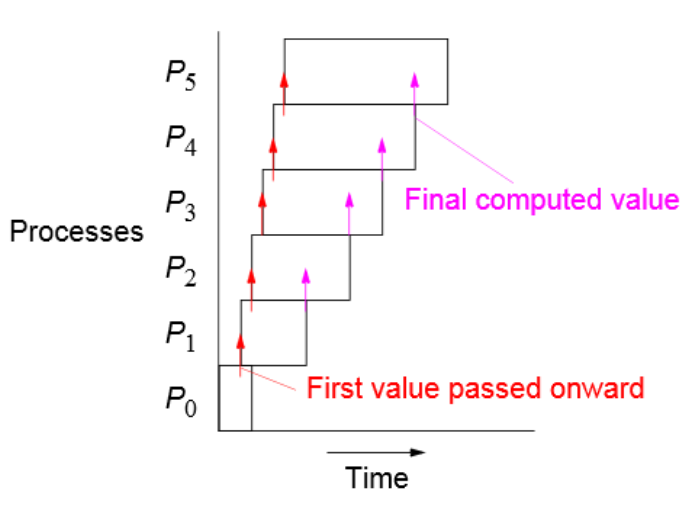
\includegraphics[width=0.5\textwidth,keepaspectratio=true]{images/pipeline.png}
				    \caption{Brief illustration of pipelined implementation of Back-Substitution Source: \cite{pipelinecomp}}
				    \label{fig:pipeline}
				\end{figure}

				For example, if core $c_{a}$ in row $a$ waits for the result of row $b$ it is no problem to factor and add all previous results of line $c, d,...$. \cite{pipelinecomp} uses this procedure for a multi core CPU, which has far better possibilities of synchronization. As already covered CUDA does not support advanced scheduling/synchronization features, except the use of atomics. But as we already know these operations produce a lot of overhead. Anyway, there will be nothing left undone and we try an attempt to port this parallelization technique to the GPU.

				The main idea behind this implementation is the following: For each value $x_i \in \vec{x}$, there exist a lock wich is \textbf{closed by default}. This lock prevents the values from being accessed too early by the other cores. When the Kernel is launched the matrix $M$ is partitioned into horizontal blocks and each block is assigned to a CUDA thread-block. As mentioned before each core waits until each element of the solution vector $\vec{x}$ unlocks and proceeds with further execution. The core with the index 0 is the first one to unlock $x_0$ after the value has been written to $\vec{x}$. All the other SMs start accessing this value immediately.

				Represents a Lock which is closed in the first place:
				\begin{lstlisting}
typedef struct Lock
{
	int	*mutex;

	Lock(){
		int state=1; //Closed to begin with!!
		checkCudaErrors(cudaMalloc((void**)&mutex,sizeof(int)));
		checkCudaErrors(cudaMemcpy(mutex, &state, sizeof(int),
						cudaMemcpyHostToDevice));
	}

	~Lock(){
		cudaFree(mutex);
	}

	__device__ void lock(){
		while(atomicCAS(mutex,0,1)!=0);
	}

	__device__ void unlock(){
		atomicExch(mutex,0);
	}

	__device__ bool is_free(){
		return atomicAnd(mutex, 1);
	}
}Lock;
				\end{lstlisting}
				As one can see this Lock consists of a constructor function, which initiates its state to closed. Furthermore a mutual exclusion is needed in order to guaranty exclusive access on the vector $\vec{x}$.
				Both atomic functions (\textbf{atomicCAS} and \textbf{atomicExch}) are necessary change and listen to the value of $mutex$.

				Implementation of pipeline Back-substitution:
				\begin{lstlisting}
#define ROUND_UP(N, S) (N%S == 0) ? N/S : N/S+1
__global__ void calc_solutions_pipeline(Lock *locks, double *d_matrix,
				size_t pitch, int var_count, double *d_solution){
	int tid = threadIdx.x,
		count,
		block_size = var_count/gridDim.x,
		start_pos;

	start_pos = (var_count-1) - block_size*blockIdx.x;
	block_size += (blockIdx.x == (gridDim.x-1))? var_count%gridDim.x : 0;
	count = var_count-(start_pos+1);
	if (blockIdx.x == 0) //first stage
	{
		for (int y = start_pos; y > start_pos-block_size; --y)
		{
			int tid_temp = tid + (var_count - blockDim.x);
			double *temp_p = (double*)((char*)d_matrix + y * pitch);
			double temp = 0;
			extern __shared__ double cache[];
			__syncthreads();

			while(BETWEEN(tid_temp, (var_count-1) - count, var_count)){
				temp += temp_p[tid_temp]*d_solution[tid_temp];
				tid_temp -= blockDim.x;
			}

			cache[threadIdx.x] = temp;
			__syncthreads();

			int i = ROUND_UP(blockDim.x, 2); //cite cuda by example page 85
			while(i > 1){
				if (threadIdx.x < i)
				{
					if (threadIdx.x +i < blockDim.x)
					{
						cache[threadIdx.x] += cache[threadIdx.x +i];
						cache[threadIdx.x +i] = 0;
					}
				} 
				__syncthreads();
				
				i = ROUND_UP(i, 2);
			}

			__syncthreads();
			count++;
		}
	} else {
		for (int y = start_pos; y > start_pos-block_size; --y)
		{
			int tid_temp = tid + (var_count - blockDim.x);
			double *temp_p = (double*)((char*)d_matrix + y * pitch);
			double temp = 0;
			extern __shared__ double cache[];
			__syncthreads();

			while(BETWEEN(tid_temp, (var_count-1) - count, var_count)){
				while (locks[tid_temp].is_free());
				
				temp += temp_p[tid_temp]*d_solution[tid_temp];
				tid_temp -= blockDim.x;
			}

			assert(threadIdx.x < blockDim.x);
			cache[threadIdx.x] = temp;
			__syncthreads();

			int i = ROUND_UP(blockDim.x, 2); //cite cuda by example page 85
			while(i > 1){
				if (threadIdx.x < i)
				{
					if (threadIdx.x +i < blockDim.x)
					{
						cache[threadIdx.x] += cache[threadIdx.x +i];
						cache[threadIdx.x +i] = 0;
					}
				}
				__syncthreads();

				i = ROUND_UP(i, 2);
			}
			__syncthreads();

			count++;
		}
	}
}
				\end{lstlisting}
				We can see that the code forks into two possibilities. As previously mentioned, the block with index 0 does not have to wait, and starts computing its first elements. As soon as other blocks see the them as \textbf{unlocked} they continue with the back substitution.

				As with the previous implementation the test results on whether pipelining the Back-substitution can actually improve performance will be given in the \textbf{Results} section.

		%\subsection{Proof}
			%In order to justify the given implementation of the forward elimination it is necessary to at least formally argue that the implementation is correct:

			%As \cite{Grcar2011163} and \cite{wiki:gaussian} report, the Gauss matrix $M$ allows several operations:
			%\begin{itemize}
				%\item Swapping rows
				%\item Swapping coulombs
				%\item Factorizing a row with $\alpha \epsilon \mathbb{R} | \alpha \neq 0$
				%\item Subtracting/Adding one row from/to another $n$ times.
			%\end{itemize}
%
			%These rules are never hurt by our parallel thread implementation, as well as the row-cyclic idea:

\chapter{Methodology For Benchmarking/Verifying The Algorithm}
	Before any test results are published, it is necessary to introduce the used test-system and the methodology behind the testing:

	\section{Hardware For Testing}
		All tests were run on the "\textbf{Pluto}" machine from the \textbf{Technical University of Vienna} which features 16 cores(\textbf{Intel Xeon E5-2650 @ 2.60GHz}) on two sockets. Each of the cores have two threads.\\
		More interesting for this thesis however, is the GPU. This system has two \textbf{NVIDIA Tesla K20Xm} GPUs which use the \textbf{Kepler} architecture.\\
		Furthermore we used a second system for comparison purpose. This machine has a \textbf{Intel Core i5-4690 @ 2.60GHz} CPU and a \textbf{NVIDIA GTX 980}. The GPU on the second system uses the "\textbf{Maxwell}" architecture which comes after Kepler. Furthermore the GTX 980 is a high end consumer oriented card that even though it is not meant for the same purpose it plays in the same field as the Tesla K20Xm.\\
		The following Tables gives a more detailed look at the used hardware:

		\begin{table}[!ht]
		\centering
		\caption{Hardware of Pluto (1)}
		\begin{tabular}{ll}
		\hline
		\multicolumn{1}{|l|}{\textbf{Core Parameters (Host)}}   & \multicolumn{1}{l|}{\textbf{Value}}                                     \\ \hline
		\multicolumn{1}{|l|}{Model Name}               & \multicolumn{1}{l|}{Intel(R) Xeon(R) CPU E5-2650 v2 @ 2.60GHz} \\ \hline
		\multicolumn{1}{|l|}{Nominal Frequency}        & \multicolumn{1}{l|}{2.6 GHz}                                   \\ \hline
		\multicolumn{1}{|l|}{CPUs}                     & \multicolumn{1}{l|}{32}                                        \\ \hline
		\multicolumn{1}{|l|}{Sockets}                  & \multicolumn{1}{l|}{2}                                         \\ \hline
		                                               &                                                                \\ \hline
		\multicolumn{1}{|l|}{\textbf{Core Parameters (Device)}} & \multicolumn{1}{l|}{\textbf{Value}}                                     \\ \hline
		\multicolumn{1}{|l|}{Model Name}               & \multicolumn{1}{l|}{NVIDIA Tesla K20Xm}                        \\ \hline
		\multicolumn{1}{|l|}{Architecture}             & \multicolumn{1}{l|}{Kepler}                                      \\ \hline
		\multicolumn{1}{|l|}{CUDA Cores}               & \multicolumn{1}{l|}{2688}                                      \\ \hline
		\multicolumn{1}{|l|}{Core Clock}               & \multicolumn{1}{l|}{706 MHz}                                   \\ \hline
		\multicolumn{1}{|l|}{Memory}                   & \multicolumn{1}{l|}{5 GB}                                      \\ \hline
		\multicolumn{1}{|l|}{Memory Clock}             & \multicolumn{1}{l|}{2.6 GHZ}                                   \\ \hline
		\end{tabular}
		\end{table}

		\begin{table}[!ht]
		\centering
		\caption{Hardware of own system (2)}
		\begin{tabular}{ll}
		\hline
		\multicolumn{1}{|l|}{\textbf{Core Parameters (Host)}}   & \multicolumn{1}{l|}{\textbf{Value}}                                  \\ \hline
		\multicolumn{1}{|l|}{Model Name}               & \multicolumn{1}{l|}{Intel(R) i5-4690 CPU @ 3.50GHz} \\ \hline
		\multicolumn{1}{|l|}{Nominal Frequency}        & \multicolumn{1}{l|}{3.5 GHz}                                \\ \hline
		\multicolumn{1}{|l|}{CPUs}                     & \multicolumn{1}{l|}{2}                                      \\ \hline
		\multicolumn{1}{|l|}{Sockets}                  & \multicolumn{1}{l|}{1}                                      \\ \hline
		                                               &                                                             \\ \hline
		\multicolumn{1}{|l|}{\textbf{Core Parameters (Device)}} & \multicolumn{1}{l|}{\textbf{Value}}                                  \\ \hline
		\multicolumn{1}{|l|}{Model Name}               & \multicolumn{1}{l|}{NVIDIA GeForce GTX 980}                 \\ \hline
		\multicolumn{1}{|l|}{Architecture}             & \multicolumn{1}{l|}{Maxwell}                                \\ \hline
		\multicolumn{1}{|l|}{CUDA Cores}               & \multicolumn{1}{l|}{2048}                                   \\ \hline
		\multicolumn{1}{|l|}{Core Clock}               & \multicolumn{1}{l|}{up to 1216 MHz}                         \\ \hline
		\multicolumn{1}{|l|}{Memory}                   & \multicolumn{1}{l|}{4 GB}                                   \\ \hline
		\multicolumn{1}{|l|}{Memory Clock}             & \multicolumn{1}{l|}{1.75 GHZ}                                  \\ \hline
		\end{tabular}
		\end{table}

	\section{Methodology For Testing}
	\label{sec:methodology_for_testing}
		The different tests are mainly done on the Pluto system except for the CPU single core performance test. Due to the much better sequential (CPU) performance of the second system it is wiser to use a system which is better optimized for sequential workload.\\
		Because the proposed implementation uses row and column wise parallelization the number of potential test cases and interesting graphs is very high, it is necessary to set certain boundaries for our test sceneries:

		For every test we generate a new input matrix with random \textbf{double (64bit)} values. As stated in ~\ref{sssec:limitations} we also have to make sure that the matrix does not contain any zero.

		When benchmarking the performance of parallel threads inside a Threadblock all tests use just one block and do not vary with matrix sizes. This test is just to show how much parallel thread power can be released with just one SM.

		Most tests are done with the use of multiple Threadblocks. For these tests we compared 2 implementations:
		\begin{itemize}
			\item The first attempt was cutting the number of parallel blocks in half and so decreasing the number of Kernel launches. We refer to this idea as "\textbf{impl 0}" in the future.
			\item The other option which was considered ("\textbf{impl 1}") just decreased the number of blocks after every iteration by one. This idea used more kernel launches but allowed more parallel cores to work at once.
		\end{itemize}

		Within these tests the number of threads per SM is set to the highest possible value. That means if just one block is used for calculation the number of its activated CUDA cores will be much higher.

		For each test we did 5 revisions in order to compensate random "noise" in the graphs. However, due to the very long time-consumption of the benchmark in section: ~\ref{sec:thread_performance_of_one_sm} we only used 3 revisions.\\
		After the benchmarking process the \textbf{mean value} of the measured results was calculated.

		Last but not least it is important to mention that we are only interested in input matrices which only produce \textbf{one} distinct solution vector otherwise we do not count this result as valid. However, this event is very unlikely and it never happened during our tests.

	\section{Verifying The Results}
		After each test it is important to check whether the computed values in the vector $\vec{x}$ are within the margin of error (0.001\%).\\
		The checker-function takes the first row of the given input Matrix $M_{i,0}$ and the solution-vector $\vec{x}$, then sums the multiplication of the corresponding values and compares it to the last element of $M_{i,0}$. Note that it is important to pass the first line of our unmodified matrix, which was randomly generated in the first place:

		Because both, the matrix and $\vec{x}$ are sill in memory of the GPU, we can launch a kernel and reuse the concept of the sum reduction to make this step faster.
		\begin{lstlisting}
#define ROUND_UP(N, S) (N%S == 0) ? N/S : N/S+1
#define DEVIATION (0.001) //in %
__global__ void check_solutions(int var_count, double *d_solution, double *d_reference){
	int tid = threadIdx.x, tid_temp;
	double dev;
	extern __shared__ double cache[];

	tid_temp = tid;
	cache[tid] = 0;
	while(tid_temp < var_count)
	{
		cache[tid] += d_reference[tid_temp] * d_solution[tid_temp];
		tid_temp+=blockDim.x;
	}
	__syncthreads();

	int i = ROUND_UP(blockDim.x, 2); //cite cuda by example page 85
	while(i > 1){
		if (tid < i)
		{
			if (tid +i < blockDim.x)
			{
				cache[tid] += cache[tid +i];
				cache[tid+i] = 0;
			}
		}
		__syncthreads();

		i = ROUND_UP(i, 2);
	}
	if(tid == 0){
		double sum = (i == 1)? cache[0]+cache[1] : cache[0];

		dev = ((d_reference[var_count] - sum)*100)*sum;
		dev = (dev < 0) ? dev*(-1) : dev;
		assert(dev < DEVIATION);
	}
}
		\end{lstlisting}

	%\subsection{Benchmarking}

\chapter{Results}
\label{ch:results}
	In this section we will revile the final test results of our implementations and compare them to each other.

	\section{Sequential Performance}
		Because the Gaussian elimination method is originally sequential we will first show how a modern CPU, which is designed to handle mostly sequential workload, handles this problem:

		\begin{figure}[!ht]
			\centering
			\begin{tikzpicture}
				\begin{axis}[
					axis lines = left,
					xlabel = size,
					ylabel = {time [seconds]}
					]
					\addplot table[col sep=comma, y=time, x=size] {graphs/cpu_bench.csv};
					\addlegendentry{CPU($n^3$)}
					\addplot table[mark=none, col sep=comma, y=time_sq, x=size] {graphs/cpu_bench.csv};
					\addlegendentry{cubic approx($n^3$)}
				\end{axis}
			\end{tikzpicture}
			\caption{Sequential Gaussian algorithm with Intel(R) i5-4690 CPU @ 3.50GHz}
		\end{figure}

		By looking at the graph above, it is noticeable that the time to calculate the solution vector $\vec{x}$ rises cubically. For comparison purposes a cubic approximation of this function was added. The CPU executes the algorithm in an acceptable time until the matrix size rises to around ~4000. So as we can see we need parallel hardware and implementation in order to delay the very strong rise of the curve further.

	\section{Thread Performance of one SM}
	\label{sec:thread_performance_of_one_sm}
		When we first started to increase performance on the GPU, we only used one Streaming Multiprocessor (= one block) and distributed the available threads horizontally on the matrix. Because one CUDA core alone is clocked far lower than a regular CPU it is reasonable to just look at the relative speedup analysis for this part:

		\begin{figure}[!ht]
			\centering
			\begin{subfigure}[t]{2\textwidth}
				\begin{tikzpicture}
					\begin{axis}[
						axis lines = left,
						xlabel = threads,
						ylabel = {Relative speedup to 1 thread}
						]
						\addplot table[
							col sep=comma,
							x=threads,
							y=speedup
							] {graphs/threads.csv};
						\legend{}
					\end{axis}
				\end{tikzpicture}
			\end{subfigure}
			\caption{Speedup that can be achieved when using multiple threads inside one SM	(Matrixsize 900)}
		\end{figure}

		The actual time that took one thread to execute the algorithm was 173 seconds. That confirms our assumption that one sequential CUDA core is by far much slower than the CPU. But one can see that if we slowly unlock the power of only one SM the speedup rises drastically to over 250. This great improvement shrinks the overall execution time to <1 second (0.62s) and can now even be compared with the CPU (0.19s).

	\section{Parallel Block Implementations}
		\subsection{Forward Elimination}
			As previously discussed a GPU consists of multiple parallel SMs which we used to implement our own version of the "\textbf{row cyclic}" implementation. Because we had to decrease the amount of Threadblocks on every iteration, we distinguished between two different procedures mentioned in ~\ref{sec:methodology_for_testing}:

			\begin{figure}[!ht]
			    \begin{subfigure}[t]{2\textwidth}
					\begin{tikzpicture}
						\begin{groupplot}[legend cell align=left, group style={group size=2 by 1}, width=0.25\textwidth, legend style={legend pos=north west,font=\tiny}]

							\nextgroupplot[
							title = {Impl 0},
							axis lines = left,
							xlabel = size,
							ylabel = {time [seconds]},
							]
							\addplot table[
								col sep=comma,
								x=size,
								y= {time 1}
								] {graphs/impl_0_inc_size.csv};
							\addlegendentry{1 SMs}

							\addplot table[
								col sep=comma,
								x=size,
								y= {time 2}
								] {graphs/impl_0_inc_size.csv};
							\addlegendentry{2 SMs}

							\addplot table[
								col sep=comma,
								x=size,
								y= {time 4}
								] {graphs/impl_0_inc_size.csv};
							\addlegendentry{4 SMs}

							\addplot table[
								col sep=comma,
								x=size,
								y= {time 8}
								] {graphs/impl_0_inc_size.csv};
							\addlegendentry{8 SMs}

							\addplot table[
								col sep=comma,
								x=size,
								y= {time 10}
								] {graphs/impl_0_inc_size.csv};
							\addlegendentry{10 SMs}

							\addplot table[
								col sep=comma,
								x=size,
								y= {time 12}
								] {graphs/impl_0_inc_size.csv};
							\addlegendentry{12 SMs}

							\addplot table[
								col sep=comma,
								x=size,
								y= {time 14}
								] {graphs/impl_0_inc_size.csv};
							\addlegendentry{14 SMs}
							\addplot table[mark=none, col sep=comma, y=time_sq, x=size] {graphs/cpu_bench.csv};
							\addlegendentry{cubic approx}

							\nextgroupplot[
							title = {Impl 1},
							axis lines = left,
							]
							\addplot table[
								col sep=comma,
								x=size,
								y= {time 1}
								] {graphs/impl_1_inc_size.csv};

							\addplot table[
								col sep=comma,
								x=size,
								y= {time 2}
								] {graphs/impl_1_inc_size.csv};

							\addplot table[
								col sep=comma,
								x=size,
								y= {time 4}
								] {graphs/impl_1_inc_size.csv};

							\addplot table[
								col sep=comma,
								x=size,
								y= {time 8}
								] {graphs/impl_1_inc_size.csv};

							\addplot table[
								col sep=comma,
								x=size,
								y= {time 10}
								] {graphs/impl_1_inc_size.csv};

							\addplot table[
								col sep=comma,
								x=size,
								y= {time 12}
								] {graphs/impl_1_inc_size.csv};

							\addplot table[
								col sep=comma,
								x=size,
								y= {time 14}
								] {graphs/impl_1_inc_size.csv};

							\addplot table[mark=none, col sep=comma, y=time_sq, x=size] {graphs/cpu_bench.csv};
						\end{groupplot}
					\end{tikzpicture}
				\end{subfigure}
				\caption{Impl 0 and 1 with variable matrix size}
			\end{figure}

			Both implementations show significant improvements in time when adding more cores but from these 2 graphs it might be difficult to tell which of them performs better.

			\begin{figure}[!ht]
				\centering
				\begin{subfigure}[t]{2\textwidth}
					\begin{tikzpicture}
						\begin{groupplot}[group style={group size=2 by 1}, width=0.25\textwidth]
						\nextgroupplot[
							title = {},
							axis lines = left,
							xlabel = cores,
							ylabel = {time [seconds]},
							ymin=50
							]
							\addplot table[
								col sep=comma,
								x=cores,
								y={time impl 0}
								] {graphs/impl_0,1_static_5500.csv};
							\addlegendentry{impl 0}

							\addplot table[
								col sep=comma,
								x=cores,
								y={time impl 1}
								] {graphs/impl_0,1_static_5500.csv};
							\addlegendentry{impl 1}

							\nextgroupplot[
							title = {},
							axis lines = left,
							ylabel = {Speedup},
							ymax = 1.6
							]
							\addplot table[
								col sep=comma,
								x=cores,
								y={Speedup 0}
								] {graphs/impl_0,1_static_5500.csv};

							\addplot table[
								col sep=comma,
								x=cores,
								y={Speedup 1}
								] {graphs/impl_0,1_static_5500.csv};
						\end{groupplot}
					\end{tikzpicture}
				\end{subfigure}
				\caption{Comparison of Impl 0 and 1 (execution time and speedup) with a constant matrix size of 5500}
				\label{fig:impl_0and1_static_5500}
			\end{figure}

			By looking at Fig: ~\ref{fig:impl_0and1_static_5500} it is noticeable that even though both impl 0 and 1 take advantage of the additional cores the second one has much more stable and smoother graphs which also affects execution time and speedup positively. From these measured values we can now conclude that greater parallelism can be preferred even though impl 1 uses more Kernel launches. So as we can see NVIDIA takes high efforts in order to make Kelnel launches very cheap. This assumption is also confirmed by \cite{Sanders:2010:CEI:1891996} and \cite{Kirk:2010:PMP:1841511}.
		
		\subsection{Back Substitution}
			So far the overall execution time of the Gaussian execution time was significantly improved by using different parallel strategies together. In the previous chapter we experimented with the idea of pipelining the back-substitution to enhance the implementation even more. As discussed before the performance results of this idea are especially interesting because it uses atomic operands for synchronization which could either help us to cut the execution time even further or result in the exact opposite.\\
			Different scenarios were tried out with both fingers crossed but unfortunately the following conclusion has to be made:

			\begin{table}[!ht]
				\centering
				\caption{Pipelined implementation VS. standard impl 1. Both use 8 blocks(SMs)}
				\label{my-label}
				\begin{tabular}{|l|l|l|}
					\hline
					\textbf{Size} & \textbf{Time pipeline {[}Seconds{]}} & \textbf{Time {[}Seconds{]}} \\ \hline
					900           & 0.53                                 & 0.53                        \\ \hline
					1000          & 0.68                                 & 0.68                        \\ \hline
					1100          & 0.85                                 & 0.84                        \\ \hline
					1200          & 1.02                                 & 1.02                        \\ \hline
					1300          & 1.22                                 & 1.21                        \\ \hline
					1400          & 1.43                                 & 1.43                        \\ \hline
					1500          & 1.65                                 & 1.65                        \\ \hline
					1800          & 2.47                                 & 2.46                        \\ \hline
					2300          & 5.18                                 & 5.17                        \\ \hline
					2500          & 6.19                                 & 6.17                        \\ \hline
					3000          & 9.22                                 & 9.2                         \\ \hline
					3200          & 12.42                                & 12.38                       \\ \hline
					3600          & 16.12                                & 16.08                       \\ \hline
					3800          & 18.01                                & 17.96                       \\ \hline
					4200          & 26.14                                & 26.09                       \\ \hline
					4500          & 30.43                                & 30.36                       \\ \hline
				\end{tabular}
			\end{table}

			Even though the pipelined attempt does not add much time to the overall results it is quite noticeable that this idea does not perform better than the sequential back substitution. It even performs worse in some sceneries. Theoretically, pipelining in this context still remains an interesting idea but in order to give it a second chance NVIDIA still has to do certain tweaks to the architecture. For example, efficient synchronization between Streaming-Multiprocessors and faster memory access.

		\section{Comparison With The Maxwell Architecture}
			As mentioned in section "\textbf{GPU Architecture}" NVIDIAs successor to Kepler was the Maxwell architecture which improved the efficiency and performance of the Steaming Multiprocessor even further.

			Even though there exist a lot of comparison results between these two generations it is still exciting to see how these improvements come into play for our implementation:

			\begin{figure}[!ht]
				\centering
				\begin{subfigure}[t]{2\textwidth}
					\begin{tikzpicture}
						\begin{groupplot}[group style={group size=2 by 1}, width=0.25\textwidth]
						\nextgroupplot[
							title = {},
							axis lines = left,
							xlabel = Streaming Multiprocessors,
							ylabel = {time [seconds]},
							]
							\addplot table[
								col sep=comma,
								x=cores,
								y={time impl 1},
								color = blue
								] {graphs/gtx_980_impl_0,1_static_5500.csv};
							\addlegendentry{GTX 980}

							\addplot table[
								col sep=comma,
								x=cores,
								y={Pluto time 1},
								color = red
								] {graphs/gtx_980_impl_0,1_static_5500.csv};
							\addlegendentry{Tesla K20Xm}

							\nextgroupplot[
							title = {},
							axis lines = left,
							ylabel = {Speedup},
							ymax = 1.6
							]
							\addplot table[
								col sep=comma,
								x=cores,
								y={Speedup 1},
								color = blue
								] {graphs/gtx_980_impl_0,1_static_5500.csv};

							\addplot table[
								col sep=comma,
								x=cores,
								y={Pluto speedup 1},
								color = red
								] {graphs/gtx_980_impl_0,1_static_5500.csv};
						\end{groupplot}
					\end{tikzpicture}
				\end{subfigure}
				\caption{Comparison of Impl 0 and 1 (execution time and speedup) with a constant matrix size(5500) using \textbf{impl 1}}
			\end{figure}

			By looking at the graph above we can see that NVIDIA did lots of improvements to their design. Surprisingly the results differ around 55-60\% in favor to the Maxwell architecture. The graphs show that while the GTX 980 does not feature as many SMs, not as much Memory and is by far more cost efficient than the Tesla K20Xm, it beats its competitor with no efforts. When it comes to speedup however, this GPU performs not as good as the Tesla.

		\section{Comparison between CPU and GPU}
			Last but not least it this section features a direct comparison between the CPU and the GPU. (Fig.: ~\ref{fig:cpu_vs_gpu_impl_1_inc_size}) We have seen that a strong CPU is needed in oder to keep the time for the execution in an acceptable amount. 

			\begin{figure}[!ht]
				\centering
				\begin{subfigure}[t]{2\textwidth}
					\begin{tikzpicture}
						\begin{axis}[
							axis lines = left,
							xlabel = size,
							ylabel = {time [seconds]},
							legend style={legend pos=north west,font=\tiny},
							legend cell align=left
							]
							\addplot table[
								col sep=comma,
								x=size,
								y={time cpu}
								] {graphs/cpu_vs_gpu_impl_1_inc_size.csv};
							\addlegendentry{CPU}

							\addplot table[
								col sep=comma,
								x=size,
								y={time 1}
								] {graphs/cpu_vs_gpu_impl_1_inc_size.csv};
							\addlegendentry{GPU 1 SMs}

							\addplot table[
								col sep=comma,
								x=size,
								y={time 2}
								] {graphs/cpu_vs_gpu_impl_1_inc_size.csv};
							\addlegendentry{GPU 2 SMs}

							\addplot table[
								col sep=comma,
								x=size,
								y={time 4}
								] {graphs/cpu_vs_gpu_impl_1_inc_size.csv};
							\addlegendentry{GPU 4 SMs}

							\addplot table[
								col sep=comma,
								x=size,
								y={time 8}
								] {graphs/cpu_vs_gpu_impl_1_inc_size.csv};
							\addlegendentry{GPU 8 SMs}

							\addplot table[mark=none, col sep=comma, y=time_sq, x=size] {graphs/cpu_bench.csv};
							\addlegendentry{cubic approx}
						\end{axis}
					\end{tikzpicture}
				\end{subfigure}
				\caption{Direct comparison: CPU vs. GPU}
				\label{fig:cpu_vs_gpu_impl_1_inc_size}
			\end{figure}
			
			It may be not surprising that the sequential CPU core quickly gets outworn by the GPU. The graph may indicate that the CPU is a bit faster than the GPU with just one enabled SM. But due to the heterogeneous Streaming Multiprocessor design the GPU will outperform the CPU in the long-run.

\chapter{Conclusion}
	As we proceed further towards the ending of this thesis we find it important to mention that applications, which heavily rely on data parallelism, will be required more and more in the future. Fluid, weather and astronomic simulations are just a few examples of tasks which can improved by using a GPU for computations instead of the CPU. The purpose of this thesis is to introduce others to the GPU architecture and give different examples on how to properly use GPUs for parallel computations.

	In order to explain the internal of a GPU NVIDIAs CUDA architecture was picked. This chapter explains what Streaming Multiprocessors are and how they function under the hood. In addition to that the different kinds of memory inside and outside the SM were introduced. We also explained how differend kinds of memory is used properly and which usage scenario suits which type best.\\
	Furthermore the CUDA API was briefly introduced and explained. Even though this thesis can not be seen as a tutorial for CUDA application developing, it provides necessary information in order to understand how CUDA functions work and which limitation it has.

	As an example we proposed a parallel implementation of the Gaussian elimination method and tried various ideas to increase the performance further. This resulted in different outcomes: For example it was possible to see positive improvements in execution time and speedup when using the proposed "\textbf{impl 1}". Unlike the pipelined approach where the use of atomic operants added too much overhead and resulted in performance loss.\\
	Even though the overall project "solving linear equations with the GPU" can be seen as a success, it is still necessary to say that the standard version of the Gaussian elimination method might not be ideal for GPU computing. This is mostly due to the lack of synchronization abilities between blocks. It was not easy to think of an implementation where barrier synchronization is not necessary. As mentioned before, our proposed implementations decrease their SM-parallelism after every iteration. This would not have been necessary if we used a more "CPU-like" architecture because it supports more advanced methods of synchronization and efficient message passing.

	As have seen how a GPU works internally and which implementations can improve performance, it is now noticeable that we only scratched the surface of the iceberg. GPU computing is a extremely complex topic which takes several years of experience for a developer to get familiar with. Therefore, I will dig further into this topic in the following years and get more experienced with the architecture as well as the API. Let the end of this thesis be the beginning of a new journey!

\chapter{Appendix: Source Code}
	\lstinputlisting[title=implementations.cu]{../implementations.cu}
	\lstinputlisting[title=resources.cu]{../resources.cu}
	
\backmatter

% Use an optional list of figures.
\listoffigures % Starred version, i.e., \listoffigures*, removes the toc entry.

% Use an optional list of tables.
\cleardoublepage % Start list of tables on the next empty right hand age.
\listoftables % Starred version, i.e., \listoftables*, removes the toc entry.

% Use an optional list of alogrithms.
\listofalgorithms
\addcontentsline{toc}{chapter}{List of Algorithms}

% Add an index.
\printindex

% Add a glossary.
\printglossaries

% Add a bibliography.
\bibliographystyle{alpha}
\bibliography{bibfile}

\end{document}